\documentclass{beamer}
\usepackage{ctex, hyperref}
\usepackage[T1]{fontenc}

% other packages
\usepackage{latexsym,amsmath,xcolor,multicol,booktabs,calligra}
\usepackage{graphicx,pstricks,listings,stackengine}

\author{userElaina}
\title{STBP 复现}
\subtitle{}
\institute{人工智能学院}
\date{2023年08月31日}
\usepackage{JilinUniv}

% defs
\def\cmd#1{\texttt{\color{red}\footnotesize $\backslash$#1}}
\def\env#1{\texttt{\color{blue}\footnotesize #1}}
\definecolor{deepblue}{rgb}{0,0,0.5}
\definecolor{deepred}{rgb}{0.6,0,0}
\definecolor{deepgreen}{rgb}{0,0.5,0}
\definecolor{halfgray}{gray}{0.55}

\lstset{
    basicstyle=\ttfamily\small,
    keywordstyle=\bfseries\color{deepblue},
    emphstyle=\ttfamily\color{deepred},    % Custom highlighting style
    stringstyle=\color{deepgreen},
    numbers=left,
    numberstyle=\small\color{halfgray},
    rulesepcolor=\color{red!20!green!20!blue!20},
    frame=shadowbox,
}

\usepackage{listings}

\lstset{
    columns=fullflexible,
    keepspaces=true,
    showspaces=false,
    showtabs=false,
    breaklines=true,
    showstringspaces=false,
    breakatwhitespace=true,
    basicstyle=\ttfamily\normalsize,
    framesep=3pt,
    xleftmargin=6pt,
    tabsize=4,
    captionpos=b
    keywordstyle        =   \bfseries,          % 关键字风格
    % commentstyle        =   \rmfamily\itshape,  % 注释的风格,斜体
    % stringstyle         =   \ttfamily,  % 字符串风格
    flexiblecolumns,                % 别问为什么,加上这个
    numbers             =   left,   % 行号的位置在左边
    showspaces          =   true,  % 是否显示空格,显示了有点乱,所以不现实了
    showstringspaces    =   true,
    frame               =   lrtb,   % 显示边框
}

\begin{document}

\kaishu
\begin{frame}
    \titlepage
    \begin{figure}[htpb]
        \begin{center}
            
\includegraphics[width=0.15\linewidth]{pic/Jilin_University_Logo.eps}
        \end{center}
    \end{figure}
\end{frame}

\begin{frame}
\tableofcontents[sectionstyle=show,subsectionstyle=show/shaded/hide,subsubsectionstyle=show/shaded/hide]
\end{frame}

\section{STBP 复现}

\begin{frame}{GPU 加速}
    \begin{itemize}
        \item pip install torch torchvision torchaudio --index-url https://download.pytorch.org/whl/cu118
        \item device = torch.device('cuda')
    \end{itemize}
\end{frame}

\begin{frame}{torch.autograd.Function}
    \begin{itemize}
        \item PyTorch 自动求导.
        \item 不可导: 需要自定义.
        \item class MyFunc(torch.autograd.Function):
        \item forward backward
    \end{itemize}
\end{frame}

\begin{frame}{torch.nn.Module}
    \begin{itemize}
        \item class MyFunc(torch.autograd.Function):
        \item forward
    \end{itemize}
\end{frame}

\begin{frame}
    \begin{figure}[l]
        \centering
        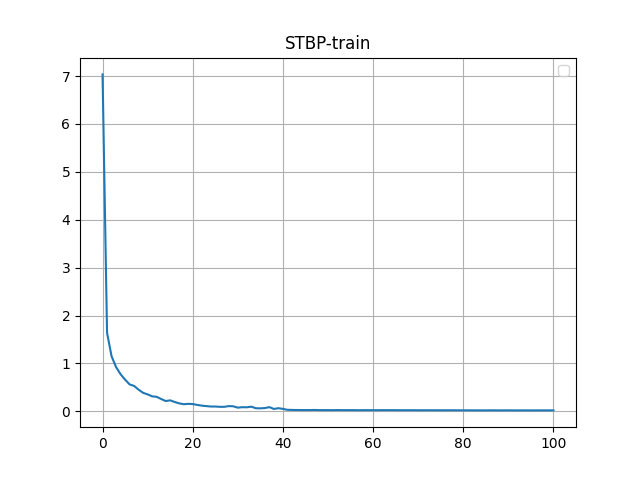
\includegraphics[height=.9\textheight]{pic/STBP-train.png}
        % \caption{基于粒子群优化的子图匹配插件}
    \end{figure}
\end{frame}

\begin{frame}
    \begin{figure}[l]
        \centering
        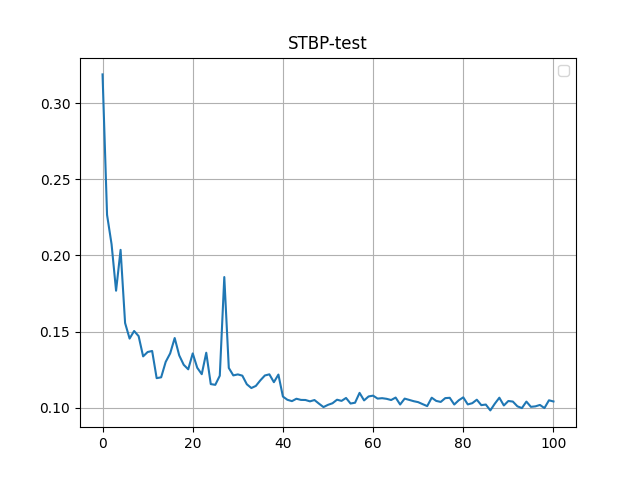
\includegraphics[height=.9\textheight]{pic/STBP-test.png}
        % \caption{基于粒子群优化的子图匹配插件}
    \end{figure}
\end{frame}

\begin{frame}
    \begin{figure}[l]
        \centering
        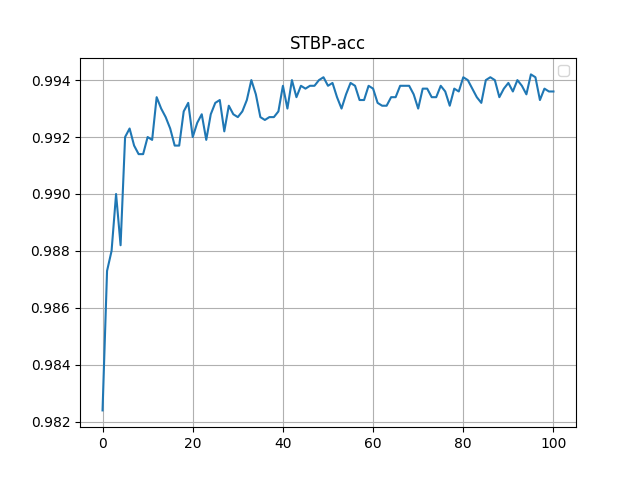
\includegraphics[height=.9\textheight]{pic/STBP-acc.png}
        % \caption{基于粒子群优化的子图匹配插件}
    \end{figure}
\end{frame}


% \begin{frame}
%     \begin{center}
%         {\Huge\calligra Thanks!}
%     \end{center}
% \end{frame}

\end{document}